\expandafter\ifx\csname ifdraft\endcsname\relax
 \begin{document}
\fi

\section{章}
\subsection{節}
texで卒業論文を書く時のテンプレートを作成した.構成は,以下の通り.
\begin{enumerate}
  \item 表紙
  \item 論文要旨
  \item 目次
  \item 典型的な章(使い回す)
  \item 参考文献
  \item 謝辞
\end{enumerate}

\subsection{表のテンプレート}
表のテンプレートを以下に示す(表\ref{tb:table_temp}).
\begin{table}[H]
  \begin{center}
   \caption{表のテンプレート}
    \label{tb:table_temp}
    \begin{tabular}{|c||c|} 
\hline
a & b  \\ \hline \hline
 	01 & 02   \\ \hline
	03 & 04   \\ \hline
    \end{tabular}
  \end{center}
\end{table}

\subsection{数式のテンプレート}
数式のテンプレートを以下に示す(式\ref{math_temp01}).
\begin{eqnarray}
\label{math_temp01}
  \mbox{\boldmath $F$} = m\mbox{\boldmath $a$}
\end{eqnarray}

数式が数行にわたる場合は以下の通り(式\ref{math_temp02}).
\begin{eqnarray}
\label{math_temp02}
  \mbox{\boldmath $\ddot{x}$} &=& \frac{\mathrm{d^2}\mbox{\boldmath $x$}}{\mathrm{d}t^2} \nonumber \\
  &=& \frac{\mathrm{d}\mbox{\boldmath $v$}}{\mathrm{d}t}
\end{eqnarray}

\subsection{引用のテンプレート}
参考にしたサイトは脇田\cite{tex_ref02}や山本\cite{tex_ref01}など.\par

\subsection{画像のテンプレート}
tempフォルダ以下のファイルの構成を以下に示す(図\ref{fig:img_temp}).
\begin{figure}[H]
  \begin{center}
    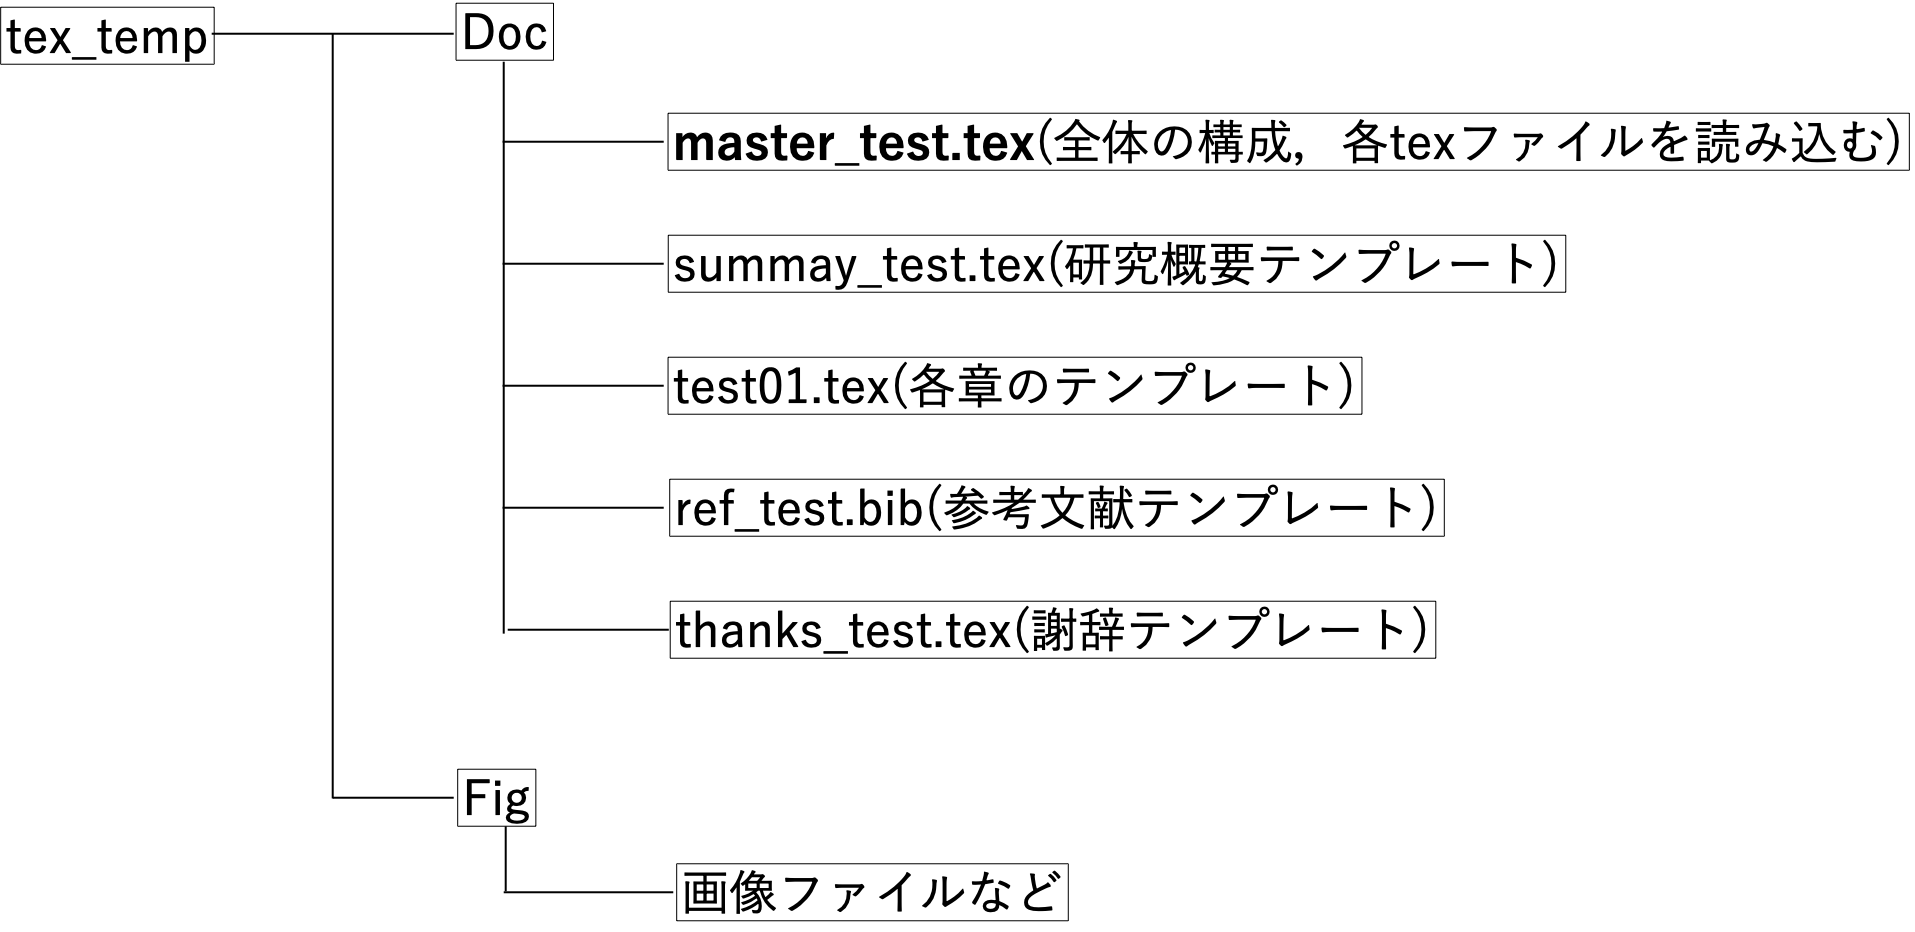
\includegraphics[keepaspectratio, scale=0.2]{../Fig/img_temp.png}
    \caption{tempフォルダ以下ののファイルの構成}
    \label{fig:img_temp}
  \end{center}
\end{figure}

\expandafter\ifx\csname ifdraft\endcsname\relax
  \end{document}
\fi
